% !TeX program = lualatex
\documentclass[../skript/main.tex]{subfiles}

\begin{document}\label{chap:hardwarearchitektur}
\chapter{Hardwarearchitektur}

\section{Worum geht es?}
Unter \textbf{Hardwarearchitektur} versteht man den grundsätzlichen Aufbau eines Rechners:
Welche Bausteine gibt es (z.\,B.\ Prozessor, Speicher, Ein-/Ausgabe), wie sind sie
\emph{organisiert} und \emph{verbunden}, und wie arbeiten sie zusammen, um Programme auszuführen?
Die heute dominierende Grundidee ist die \textbf{von-Neumann-Architektur}.

\section{John von Neumann und die Grundidee}
In den 1940er Jahren formulierte John von Neumann (gemeinsam mit weiteren Pionieren um ENIAC/EDVAC)
eine einfache, aber revolutionäre Idee: \textbf{Programm und Daten liegen im gleichen Speicher.}
Das heißt, ein Programm ist selbst nur eine Folge von Zahlen (Maschinenbefehlen), die genau wie Daten
im Hauptspeicher abgelegt und von der CPU geholt werden. Diese \emph{Stored-Program}-Idee macht
Rechner \emph{flexibel} (beliebige Programme ladbar) und \emph{universell}.

\subsection*{Bausteine im von-Neumann-Modell}
\begin{itemize}
	\item \textbf{CPU (Prozessor)} mit
	\begin{itemize}
		\item \textbf{Steuerwerk} (kontrolliert den Ablauf, interpretiert Befehle),
		\item \textbf{Rechenwerk/ALU} (führt Operationen wie Addieren, Vergleichen aus),
		\item \textbf{Registern} (kleinste, sehr schnelle Speicherplätze, z.\,B.\ Akkumulator, Program Counter).
	\end{itemize}
	\item \textbf{Hauptspeicher (RAM)}: enthält \emph{sowohl} Daten \emph{als auch} Befehle.
	\item \textbf{Ein-/Ausgabe (I/O)}: Tastatur, Bildschirm, Netz, Sensoren, Aktoren \dots
	\item \textbf{Bus-System}: Verbindet die Bausteine (Adress-, Daten- und Steuerbus).
\end{itemize}

\begin{figure}[H]
	\centering
	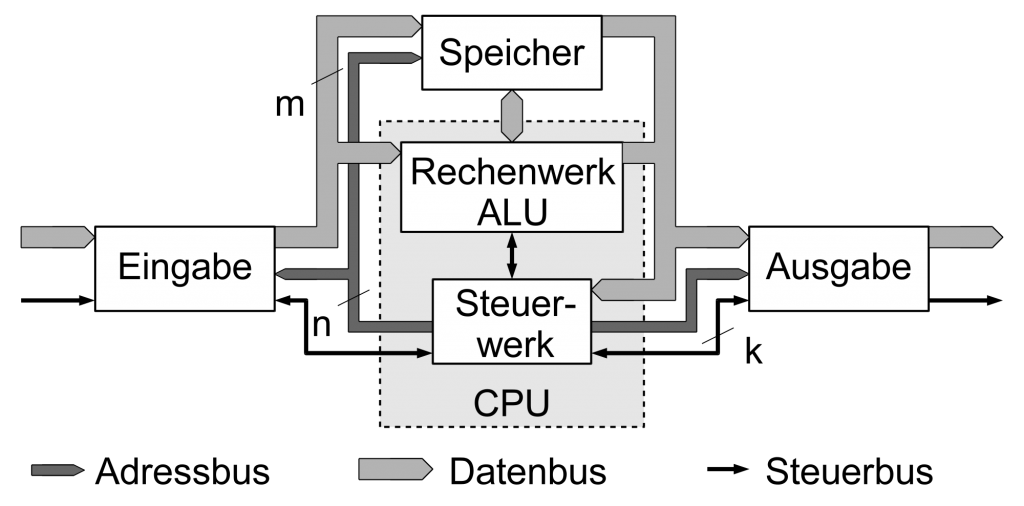
\includegraphics[width=.75\textwidth]{vonNeumannarchitektur.png}
	\caption{Architektur von Neumann Rechners.}
	\label{fig:vonNeumannarchitektur}
\end{figure}
%\begin{figure}[H]
%	\centering
%	\setlength{\fboxsep}{6pt}
%	\begin{tabular}{c}
%		\fbox{\parbox{0.8\textwidth}{\centering Ein-/Ausgabe (I/O)}}\\[0.5em]
%		$\updownarrow$ \emph{Bus-System} \\[0.5em]
%		\fbox{\parbox{0.8\textwidth}{\centering Hauptspeicher (Programme \& Daten)}}\\[0.5em]
%		$\updownarrow$ \emph{Bus-System} \\[0.5em]
%		\fbox{\parbox{0.8\textwidth}{\centering CPU = Steuerwerk + ALU + Register}}
%	\end{tabular}
%	\caption{Vereinfachtes von-Neumann-Modell.}
%\end{figure}

\section{Der Befehlszyklus (Fetch–Decode–Execute)}
Jeder Maschinenbefehl läuft in drei Schritten durch die CPU:
\begin{enumerate}
	\item \textbf{Fetch} (Holen): Der \emph{Program Counter (PC)} zeigt auf die nächste Befehlsadresse.
	Der Befehl wird aus dem Speicher gelesen und in das \emph{Befehlsregister (IR)} gelegt.
	\item \textbf{Decode} (Dekodieren): Das Steuerwerk „versteht“, welcher Operationstyp gemeint ist
	(z.\,B.\ ADD, LOAD, STORE) und welche Operanden/Adressen beteiligt sind.
	\item \textbf{Execute} (Ausführen): Die ALU rechnet bzw.\ I/O/Speicherzugriffe passieren.
	Der PC wird auf den nächsten Befehl gesetzt (oder bei Sprüngen angepasst).
\end{enumerate}

\paragraph{Mini-Beispiel (gedankliches Maschinenprogramm).}
\begin{lstlisting}[caption={Addition zweier Speicherstellen und Ablage des Ergebnisses}]
	LOAD R0, [x]   ; lade x in Register R0
	LOAD R1, [y]   ; lade y in Register R1
	ADD  R0, R1    ; R0 := R0 + R1
	STORE R0, [z]  ; speichere Ergebnis in z
\end{lstlisting}
Hier holt die CPU nacheinander die Befehle (Fetch), dekodiert sie (Decode) und führt sie aus (Execute).

\section{Speicher, Wortbreite und Adressierung}
\begin{itemize}
	\item \textbf{Wortbreite} (z.\,B.\ 32 Bit, 64 Bit) gibt an, wie viele Bits die CPU in einem Schritt besonders effizient verarbeitet
	(Register- und ALU-Breite). Sie beeinflusst u.\,a.\ den darstellbaren Adressraum und Zahlenbereich.
	\item \textbf{Adressbus/Datenbus}: Mit \(n\) Adressleitungen kann man \(2^n\) Speicheradressen ansprechen.
	\item \textbf{Speicherhierarchie}: Register \(\rightarrow\) Caches (L1/L2/L3) \(\rightarrow\) RAM \(\rightarrow\) SSD/HDD.
	Je näher an der CPU, desto schneller (aber kleiner/teurer).
\end{itemize}

\section{Warum ist das so erfolgreich?}
\begin{itemize}
	\item \textbf{Einfachheit}: Ein einheitlicher Speicher für Programme und Daten macht die Hardware und das Laden von Programmen einfach.
	\item \textbf{Flexibilität}: Beliebige Programme können nachgeladen werden; Selbstmodifizierender Code ist (theoretisch) möglich.
	\item \textbf{Universalität}: Mit genug Speicher und Zeit kann ein solcher Rechner jede berechenbare Aufgabe lösen (Church–Turing-Idee).
\end{itemize}

\section{Grenzen: der Von-Neumann-Flaschenhals}
Weil \emph{Programm} und \emph{Daten} über \emph{denselben} Speicher-/Busweg kommen, konkurrieren sie um Bandbreite.
Das bremst: Die CPU könnte schneller rechnen, als Daten/Befehle nachgeliefert werden. Was hilft dagegen?

\begin{itemize}
	\item \textbf{Caches (Zwischenspeicher):} Kleine, sehr schnelle Speicher \emph{in der CPU}, die oft gebrauchte Daten/Befehle bereithalten. % (wie ein Spickzettel direkt am Platz)
	\item \textbf{Vorabruf (Prefetch):} Die CPU \emph{holt schon vorher}, was sie gleich brauchen wird. % (wie Vorräte rechtzeitig aus dem Keller holen)
	\item \textbf{Pipelining (Fließband):} Eine Instruktion wird in Schritte zerlegt; mehrere Instruktionen sind gleichzeitig in \emph{verschiedenen} Schritten. % (wie Autos gleichzeitig in Waschen, Trocknen, Polieren)
	\item \textbf{Superskalar (mehrere Einheiten):} Die CPU kann \emph{mehr als einen} Befehl pro Takt starten. % (wie mehrere Kassen, nicht nur eine)
	\item \textbf{Mehr Kerne (Multi-Core):} Mehrere Rechenkerne arbeiten \emph{parallel} an unterschiedlichen Aufgaben. % (Teamarbeit statt Einzelkämpfer)
	\item \textbf{Vektoreinheiten (SIMD):} \emph{Eine} Rechenanweisung auf \emph{viele} Daten gleichzeitig ausführen. % (eine Schablone, viele Teile auf einmal)
	\item \textbf{Breitere/ schnellere Verbindungen:} Mehr Bits pro Takt (\emph{breiter Bus}) und schnellerer Speicher (z.\,B. DDR, HBM) liefern Daten zügiger. % (mehr Fahrspuren und höhere Geschwindigkeit)
\end{itemize}

\begin{quote}\small
	\textbf{Merksatz:} Wenn die CPU warten muss, helfen \emph{nähere Vorräte} (Cache), \emph{rechtzeitig holen} (Prefetch), \emph{gleichzeitig arbeiten} (Pipeline/parallel), und \emph{breitere/schnellere Wege} (Bus/Speicher).
\end{quote}


\section{Harvard vs.\ von Neumann (und die Praxis heute)}
Die \textbf{Harvard-Architektur} trennt \emph{Befehls-} und \emph{Datenspeicher} (je eigener Bus).
Vorteil: Gleichzeitige Zugriffe, kein Flaschenhals an dieser Stelle. Viele \emph{Mikrocontroller/DSPs}
und auch \emph{moderne CPUs intern} nutzen eine \textbf{modifizierte Harvard-Architektur}:
z.\,B.\ getrennte \emph{Instruktions-} und \emph{Datencaches}, obwohl der \emph{Hauptspeicher} gemeinsam ist.
Damit kombiniert man die Programmierfreundlichkeit des von-Neumann-Modells mit Leistungsgewinnen.

	
\end{document}